%%%%%%%%%%%%%%%%%%%%%%%%%%%%%%%%%%%%%%%%%%%%%%%%%%%%%%%%%%%%%%%%%%%%%%%%%%%%%%%%%%
\begin{frame}[fragile]\frametitle{}
\begin{center}
{\Large Introduction}
\end{center}
\end{frame}


%%%%%%%%%%%%%%%%%%%%%%%%%%%%%%%%%%%%%%%%%%%%%%%%%%%%%%%%%%%
\begin{frame}[fragile]\frametitle{Current State}
\begin{itemize}
\item 44\% of US workforce $<$ \$18K/yr ($<$ poverty line), works 80-100 hrs/week
\item Automation CAGR 7\% (as per BCG), to reach \$114B by 2025
\end{itemize}

\begin{center}
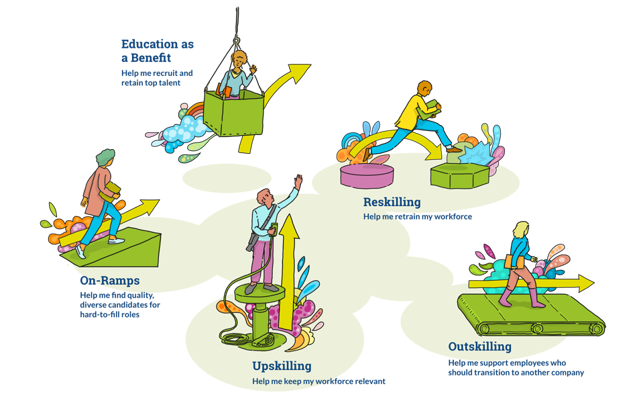
\includegraphics[width=0.8\linewidth,keepaspectratio]{career1}
\end{center}

{\tiny (Ref: As Pressure To Upskill Grows, 5 Models Emerge – Forbs.com)}
\end{frame}


%%%%%%%%%%%%%%%%%%%%%%%%%%%%%%%%%%%%%%%%%%%%%%%%%%%%%%%%%%%
\begin{frame}[fragile]\frametitle{McKinsey Global Institute Report – Discussion Paper 2018}



\begin{center}
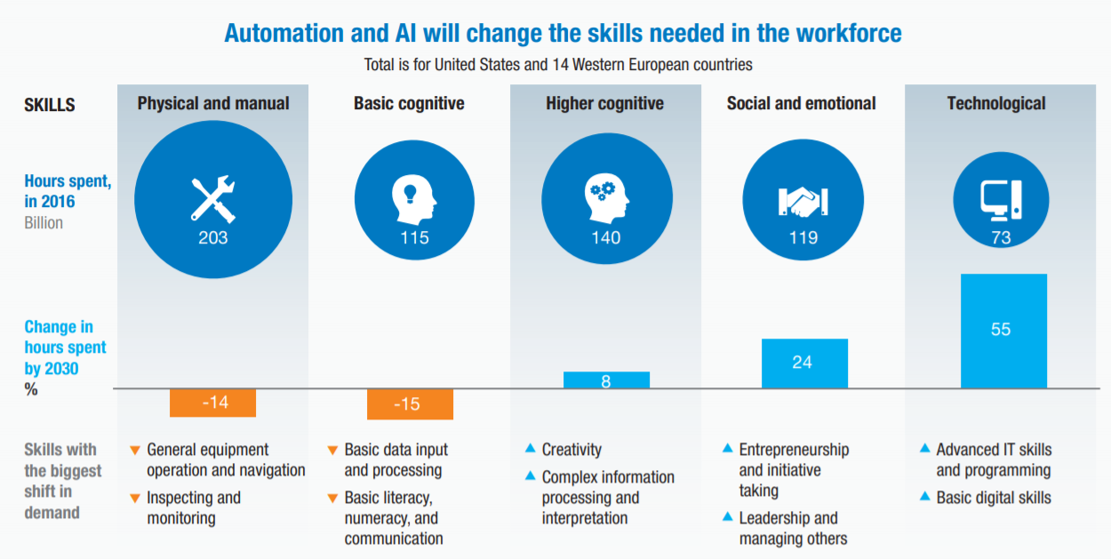
\includegraphics[width=\linewidth,keepaspectratio]{career2}
\end{center}

\end{frame}



%%%%%%%%%%%%%%%%%%%%%%%%%%%%%%%%%%%%%%%%%%%%%%%%%%%%%%%%%%%
\begin{frame}[fragile]\frametitle{Examples}
\begin{columns}
    \begin{column}[T]{0.5\linewidth}
		Less mechanical, automatable

      \begin{itemize}
		\item Bill and account collectors
		\item Data entry operators
		\item Computer network support 
		\item Secretaries and administrative assistants
		\item Insurance sales agents
		\item Office clerks

	  \end{itemize}
\begin{center}
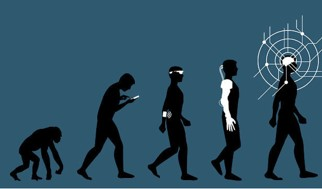
\includegraphics[width=0.8\linewidth,keepaspectratio]{career3}
\end{center}

{\tiny (Source: The Simplistic Debate Over Artificial Intelligence – Preston Estep
)}

    \end{column}
    \begin{column}[T]{0.5\linewidth}
		More Cognitive, Creative, Human

      \begin{itemize}
		\item Software developers
		\item Customer service representatives
		\item General and operations managers
		\item Human resources managers
		\item Personal finance advisors
		\item Psychologists
		\item Artists
		\item Sportsman
		\item Researchers
		\item Nurses, care

	  \end{itemize}
    \end{column}
  \end{columns}
\end{frame}


%%%%%%%%%%%%%%%%%%%%%%%%%%%%%%%%%%%%%%%%%%%%%%%%%%%%%%%%%%%
\begin{frame}[fragile]\frametitle{Changes}
\begin{columns}
    \begin{column}[T]{0.5\linewidth}
			Technological
      \begin{itemize}
			\item AI deluge
			\item Digitization $\rightarrow$ Data + APIs
			\item Remote *
			\end{itemize}
			
			Social
      \begin{itemize}
			\item Over interaction + isolation
			\item Obsolete roles, emergence of new
			\item Lifelong re-skilling
			\end{itemize}			


    \end{column}
    \begin{column}[T]{0.5\linewidth}
\begin{center}
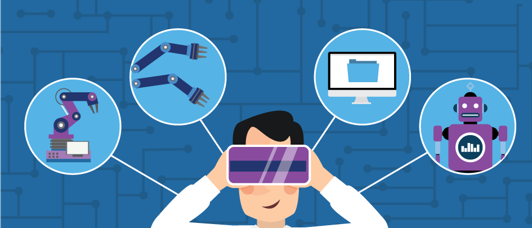
\includegraphics[width=0.8\linewidth,keepaspectratio]{career4}
\end{center}

{\tiny (Source: Rise of the Chatbots: How AI Changed Customer Service – Salesforce.com)}

		Financial
      \begin{itemize}
			\item Widening gap
			\item Flatter world
			\item Gigs over jobs
			\end{itemize}
    \end{column}
  \end{columns}
\end{frame}


%%%%%%%%%%%%%%%%%%%%%%%%%%%%%%%%%%%%%%%%%%%%%%%%%%%%%%%%%%%
\begin{frame}[fragile]\frametitle{Examples}
\begin{columns}
    \begin{column}[T]{0.5\linewidth}
			Technological
      \begin{itemize}
			\item AI deluge
			\item Digitization $\rightarrow$ Data + APIs
			\item Remote *
			\end{itemize}
    \end{column}
    \begin{column}[T]{0.5\linewidth}
			Social
      \begin{itemize}
			\item Over interaction + isolation
			\item Obsolete roles, emergence of new
			\item Lifelong re-skilling
			\end{itemize}		
    \end{column}
  \end{columns}
	
	\begin{center}
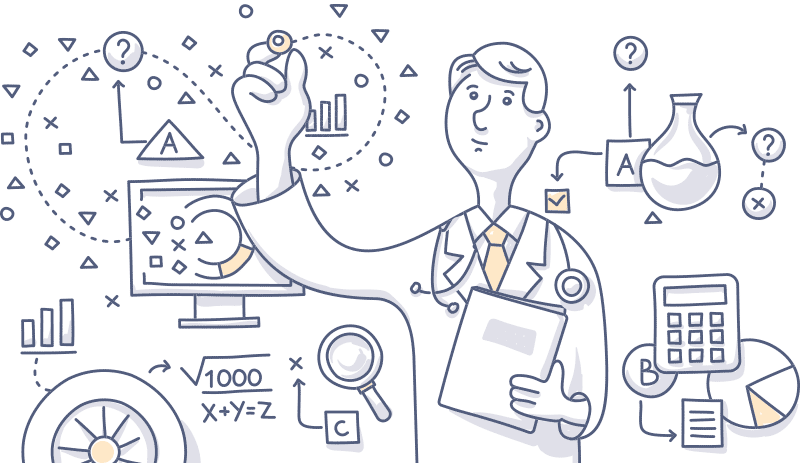
\includegraphics[width=0.6\linewidth,keepaspectratio]{career5}
\end{center}

{\tiny (Source: AI in healthcare – foreseemed.com)}

\end{frame}

%%%%%%%%%%%%%%%%%%%%%%%%%%%%%%%%%%%%%%%%%%%%%%%%%%%%%%%%%%%
\begin{frame}[fragile]\frametitle{Examples}
	
	\begin{center}
	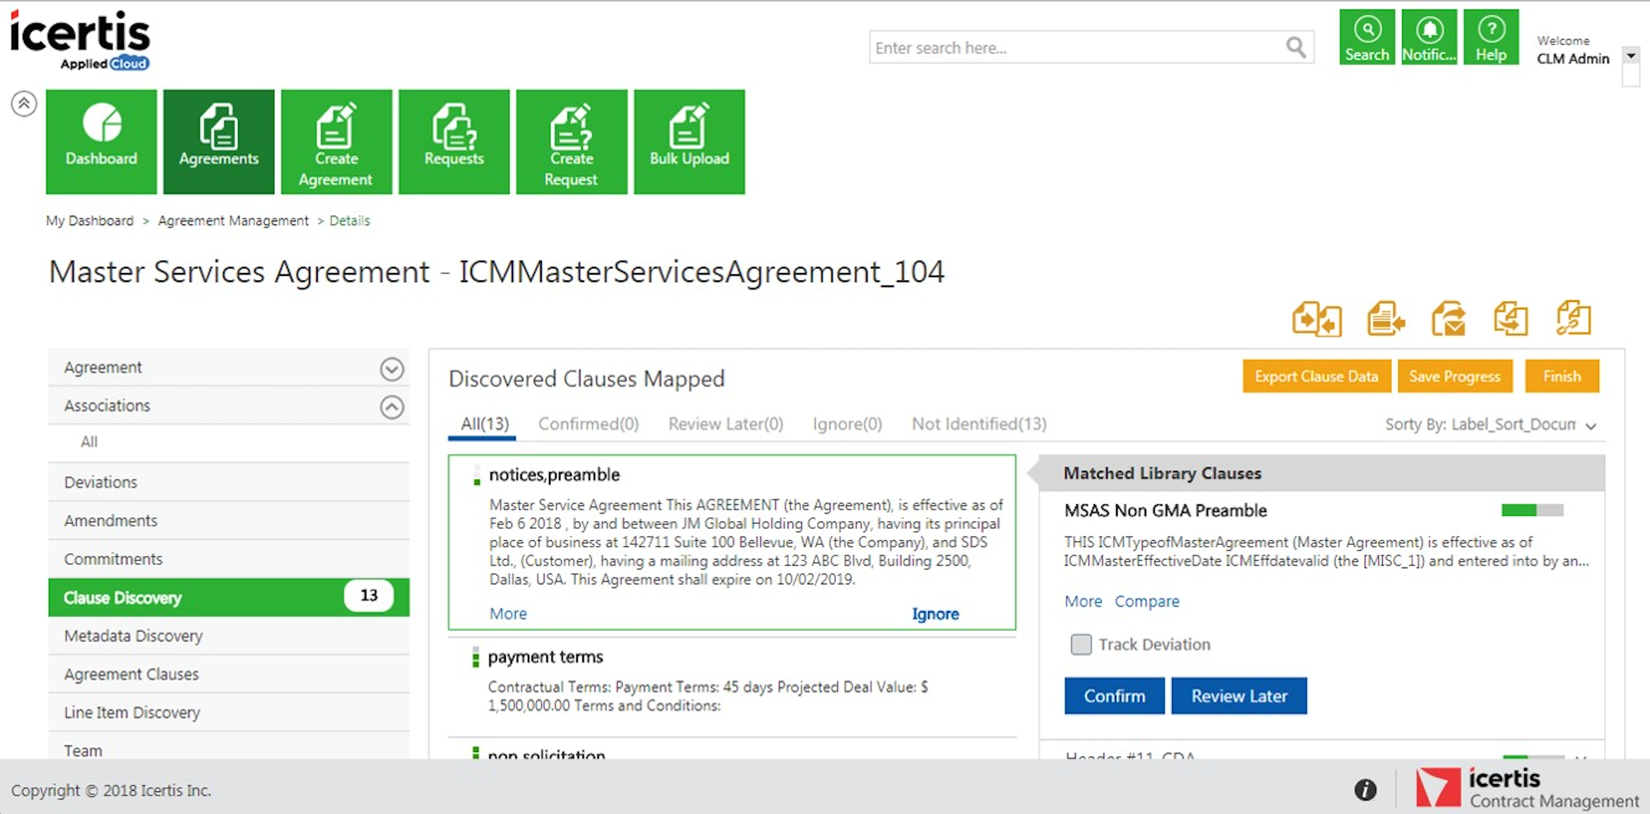
\includegraphics[width=\linewidth,keepaspectratio]{career6}
	\end{center}

\end{frame}

%%%%%%%%%%%%%%%%%%%%%%%%%%%%%%%%%%%%%%%%%%%%%%%%%%%%%%%%%%%%%%%%%%%%%%%%%%%%%%%%%%
\begin{frame}[fragile]\frametitle{}
\begin{center}
{\Large Data Science is critical in bringing intelligent automation}
\end{center}
\end{frame}


%%%%%%%%%%%%%%%%%%%%%%%%%%%%%%%%%%%%%%%%%%%%%%%%%%%%%%%%%%%%%%%%%%%%%%%%%%%%%%%%%%
\begin{frame}[fragile]\frametitle{}
\begin{center}
{\Large What are Data Sciences? \\ \small ie What is Artificial Intelligence? Machine Learning? Deep Learning?}
\end{center}
\end{frame}


%%%%%%%%%%%%%%%%%%%%%%%%%%%%%%%%%%%%%%%%%%%%%%%%%%%%%%%%%%%
\begin{frame}[fragile]\frametitle{Data Science}

\begin{itemize}
\item Science of Data (obviously)
\item Use of Data for Applications
\item Some parts of AI uses Data to find patterns and insights which are helpful in multuple applicatons
\item Machine and Deep Learning that part of AI that leverages data.
\end{itemize}

So, more on AI-ML here \ldots

\end{frame}


%%%%%%%%%%%%%%%%%%%%%%%%%%%%%%%%%%%%%%%%%%%%%%%%%%%%%%%%%%%%%%%%%%%%%%%%%%%%%%%%%%
\begin{frame}[fragile]\frametitle{}
\begin{center}
{\Large ''Houston, we have a problem!!''}
\end{center}
\end{frame}

%%%%%%%%%%%%%%%%%%%%%%%%%%%%%%%%%%%%%%%%%%%%%%%%%%%%%%%%%%%
\begin{frame}[fragile]\frametitle{The Problem}

\begin{itemize}
\item Every company is claiming to be working in AI-ML
\begin{itemize}
\item Is it so?
\item What exactly is AI (ML)?
\item What is not AI?
\end{itemize}

\item Or is it just a plain BIG hype?

\end{itemize}
	  
\end{frame}


%%%%%%%%%%%%%%%%%%%%%%%%%%%%%%%%%%%%%%%%%%%%%%%%%%%%%%%%%%%%%%%%%%%%%%%%%%%%%%%%%%
\begin{frame}[fragile]\frametitle{What's the core idea?'}
\begin{itemize}
\item behind problem solving?
\item behind writing software algorithms?
\item solving research problems?
\end{itemize}
\end{frame}

%%%%%%%%%%%%%%%%%%%%%%%%%%%%%%%%%%%%%%%%%%%%%%%%%%%%%%%%%%%
\begin{frame}[fragile]\frametitle{Desire}
\begin{itemize}
\item To find a ``function''
\item To find a relation
\item To find a transformation
\item To build a model
\item From given inputs to desired outputs.
\end{itemize}
That's it.
\end{frame}

%%%%%%%%%%%%%%%%%%%%%%%%%%%%%%%%%%%%%%%%%%%%%%%%%%%%%%%%%%%
\begin{frame}[fragile]\frametitle{Functions}
\begin{itemize}
\item Some functions are straight forward
\item {\em ``In summer, ice-cream sale goes up''}
\item Cause and effect
\item Relation (function, Mathematical model) is found out
\item Here, simple rule based programming suffices
\end{itemize}
\end{frame}

%%%%%%%%%%%%%%%%%%%%%%%%%%%%%%%%%%%%%%%%%%%%%%%%%%%%%%%%%%%
\begin{frame}[fragile]\frametitle{Functions}
\begin{itemize}
\item But some functions are complex
\item {\em ``More you put efforts, your business flourishes.''}
\item Cause and effect again, but the relation is far to complex
\item Too many variables
\item Here, simple rule based programming not humanly possible.
\item Lots of research needed to come up with equations.
\end{itemize}
\end{frame}

%%%%%%%%%%%%%%%%%%%%%%%%%%%%%%%%%%%%%%%%%%%%%%%%%%%%%%%%%%%
\begin{frame}[fragile]\frametitle{Functions}
\begin{itemize}
\item $E = mc^2$
\item What's this? a function?
\item Input variable(s)?
\item Output variable(s)?
\item Parameters?
\item How's the relation? linear?
\end{itemize}
\end{frame}



%%%%%%%%%%%%%%%%%%%%%%%%%%%%%%%%%%%%%%%%%%%%%%%%%%%%%%%%%%%
\begin{frame}[fragile]\frametitle{Functions}
\begin{itemize}
\item But most real-life functions are not deterministic
\item Some are probabilistic, some non-linear.
\item {\em ``Detecting if the tumor is benign or malignant''}
\item {\em ``At any state in the game of chess, whats the next move?''}
\end{itemize}
\end{frame}

%%%%%%%%%%%%%%%%%%%%%%%%%%%%%%%%%%%%%%%%%%%%%%%%%%%%%%%%%%%
\begin{frame}[fragile]\frametitle{Chess: next move?}
\begin{itemize}
\item Needs extreme expertise
\item Needs ``intelligence''
\item How do you get that?
\begin{itemize}
\item Built by lots of training.
\item By studying lots of past games.
\end{itemize}
\item This is how Humans build intelligence
\end{itemize}
\end{frame}

%%%%%%%%%%%%%%%%%%%%%%%%%%%%%%%%%%%%%%%%%%%%%%%%%%%%%%%%%%%
\begin{frame}[fragile]\frametitle{Intelligence}
\begin{itemize}
\item Can machine (software/program) also do the same?
\item Can it play chess?
\item Can it build intelligence?
\item By looking at past experiences (data), 
\item Training Data: games played, moves used, etc.
\end{itemize}
Yes, it can!! Thats Artificial Intelligence.
\end{frame}

%%%%%%%%%%%%%%%%%%%%%%%%%%%%%%%%%%%%%%%%%%%%%%%%%%%%%%%%%%%%%%%%%%%%%%%%%%%%%%%%%%
\begin{frame}[fragile]\frametitle{}
\begin{center}
{\Large What is AI?}
\end{center}
\end{frame}



%%%%%%%%%%%%%%%%%%%%%%%%%%%%%%%%%%%%%%%%%%%%%%%%%%%%%%%%%%%
\begin{frame}[fragile]\frametitle{ What is Artificial Intelligence (AI)?}
My definition:


``If machines (or computer programs) start doing some/all of these ``intelligent'' tasks, then that's Artificial Intelligence''

\end{frame}

%%%%%%%%%%%%%%%%%%%%%%%%%%%%%%%%%%%%%%%%%%%%%%%%%%%%%%%%%%%
\begin{frame}[fragile]\frametitle{ Intelligence: the differentiation}
\begin{itemize}
\item Ability to think various domains
\item Ability produce something new
\item Ability to detect the unseen
\item Ability to enhance knowledge (rules, patterns)
\end{itemize}
All these, AI has started doing. The AI era has arrived!!
\end{frame}



%%%%%%%%%%%%%%%%%%%%%%%%%%%%%%%%%%%%%%%%%%%%%%%%%%%%%%%%%%%
\begin{frame}[fragile]\frametitle{Everyday usage}
Artificial intelligence seems to have become ubiquitous.
\begin{itemize}
\item Replying to our emails on Gmail
\item Learning how to drive our cars,
\item Sorting our holiday photos.
\item etc.
\end{itemize}
Too good to be true, isn't it, sort of Magical !!
\end{frame}

%%%%%%%%%%%%%%%%%%%%%%%%%%%%%%%%%%%%%%%%%%%%%%%%%%%%%%%%%%%
\begin{frame}[fragile]\frametitle{But then \ldots}
\begin{itemize}
\item When its too good, you start suspecting
\item Is it for real!!
\item How can such thing happen?
\item How far will it go?
\end{itemize}
The next thing you know, people are worrying about exactly how and when AI is going to doom humanity.
\end{frame}


%%%%%%%%%%%%%%%%%%%%%%%%%%%%%%%%%%%%%%%%%%%%%%%%%%%%%%%%%%%
\begin{frame}[fragile]\frametitle{Relationship between AI, ML, DL}
\begin{center}
\includegraphics[width=\linewidth,keepaspectratio]{ai1}
\end{center}
{\tiny (Ref: https://blogs.nvidia.com/blog/2016/07/29/whats-difference-artificial-intelligence-machine-learning-deep-learning-ai/)}
\end{frame}




%%%%%%%%%%%%%%%%%%%%%%%%%%%%%%%%%%%%%%%%%%%%%%%%%%%%%%%%%%%
\begin{frame}[fragile]\frametitle{Traditional vs. Machine Learning?}
\begin{center}
\includegraphics[width=0.8\linewidth,keepaspectratio]{tradml}
\end{center}
\end{frame}

%%%%%%%%%%%%%%%%%%%%%%%%%%%%%%%%%%%%%%%%%%%%%%%%%%%%%%%%%%%
\begin{frame}[fragile]\frametitle{Why Machine Learning?}
\begin{itemize}
\item Problems with High Dimensionality
\item Hard/Expensive to program manually
\item Techniques to model `ANY' function given `ENOUGH' data.
\item Job \$\$\$
\end{itemize}
%\begin{center}
%\includegraphics[width=0.45\linewidth,keepaspectratio]{hp}
%\end{center}
\end{frame}



%%%%%%%%%%%%%%%%%%%%%%%%%%%%%%%%%%%%%%%%%%%%%%%%%%%%%%%%%%%
\begin{frame}[fragile]\frametitle{Why now?}
\begin{itemize}
\item Flood of data (Internet, IoT)
\item Increasing computational power
\item Easy/free availability of algorithms 
\item Increasing support from industries
\end{itemize}
\end{frame}

%%%%%%%%%%%%%%%%%%%%%%%%%%%%%%%%%%%%%%%%%%%%%%%%%%%%%%%%%%%%%%%%%%%%%%%%%%%%%%%%%%
\begin{frame}[fragile]\frametitle{}
\begin{center}
{\Large Preparing Career in Data Sciences}
\end{center}
\end{frame}

%%%%%%%%%%%%%%%%%%%%%%%%%%%%%%%%%%%%%%%%%%%%%%%%%%%%%%%%%%%
\begin{frame}[fragile]\frametitle{So, What is a Data Scientist?}
\begin{itemize}
\item Software + Mathematics + ML/DL specific techniques
\item Discovers patterns and trends in datasets to get insights.
\item Creates forecasting algorithms like Classification, Clustering, etc
\end{itemize}
\end{frame}

%%%%%%%%%%%%%%%%%%%%%%%%%%%%%%%%%%%%%%%%%%%%%%%%%%%%%%%%%%%
\begin{frame}[fragile]\frametitle{Business Intelligence vs Data Science}
\begin{table}[]
\begin{tabular}{p{0.4\textwidth}p{0.4\textwidth}}
\hline
{\bf Business Intelligence} & {\bf Data Science}         	\\ \hline
Extract insights using past data    & Predict future using past data       		\\ \hline
Uses structured data      & Uses both structured and unstructured data  				\\ \hline
Use of basic statistics with emphasis on visualization (dashboards, reports)    & Leverages more sophisticated statistical and predictive analysis and machine learning (ML)            	\\ \hline
\end{tabular}
\end{table}
\end{frame}

%%%%%%%%%%%%%%%%%%%%%%%%%%%%%%%%%%%%%%%%%%%%%%%%%%%%%%%%%%%
\begin{frame}[fragile]\frametitle{Roles in Data Science}
\begin{itemize}
\item Researcher: Advanced Mathematics, Programming, domain, Adv ML/DL, etc. You invent new things and write NeurIPS paper.
\item Implementation:
	\begin{itemize}
	\item Data Analyst: Bridge the gap between the data scientists and the business analysts, organizing and analyzing data to answer the questions the organization poses. 
	\item Data Engineer: Focus on developing, deploying, managing, and optimizing the organization’s data infrastructure and data pipelines.
	\item Data Scientist: Use/mine data, clean, build applications, reports, etc
	\end{itemize}
\item User level: Product Manager, Sales, Manager, etc
\end{itemize}
\end{frame}

%%%%%%%%%%%%%%%%%%%%%%%%%%%%%%%%%%%%%%%%%%%%%%%%%%%%%%%%%%%
\begin{frame}[fragile]\frametitle{}
	
	\begin{center}
	{\Large But \ldots, But \ldots, How to prepare?}  
	\end{center}

\end{frame}

%%%%%%%%%%%%%%%%%%%%%%%%%%%%%%%%%%%%%%%%%%%%%%%%%%%%%%%%%%%
\begin{frame}[fragile]\frametitle{}
	
	\begin{center}
	{\Large What got you here,  won’t get you there!!} \\
	{\bf - Marshal Goldsmith}
	\end{center}

\end{frame}

%%%%%%%%%%%%%%%%%%%%%%%%%%%%%%%%%%%%%%%%%%%%%%%%%%%%%%%%%%%
\begin{frame}[fragile]\frametitle{}
	
	\begin{center}
	{\Large So, Well, you can’t prepare!!}  \\
	
	not everything, but certainly, specifically \ldots
	\end{center}

\end{frame}

%%%%%%%%%%%%%%%%%%%%%%%%%%%%%%%%%%%%%%%%%%%%%%%%%%%%%%%%%%%
\begin{frame}[fragile]\frametitle{Upwinds}
	
	\begin{center}
	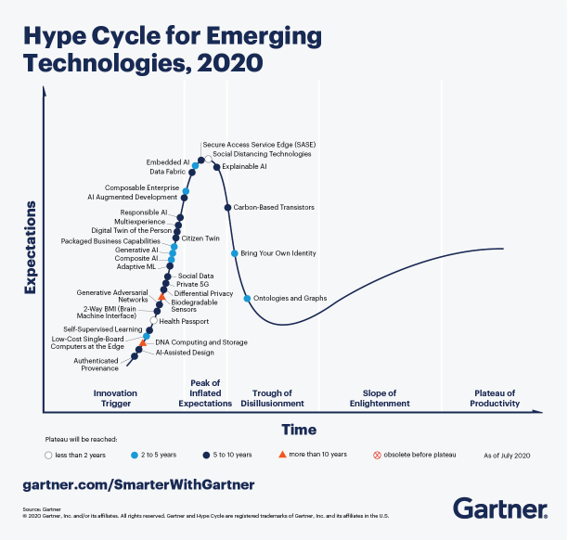
\includegraphics[width=0.8\linewidth,keepaspectratio]{career7}
	\end{center}

\end{frame}

%%%%%%%%%%%%%%%%%%%%%%%%%%%%%%%%%%%%%%%%%%%%%%%%%%%%%%%%%%%
\begin{frame}[fragile]\frametitle{Specialization is the key}
	
	\begin{center}
	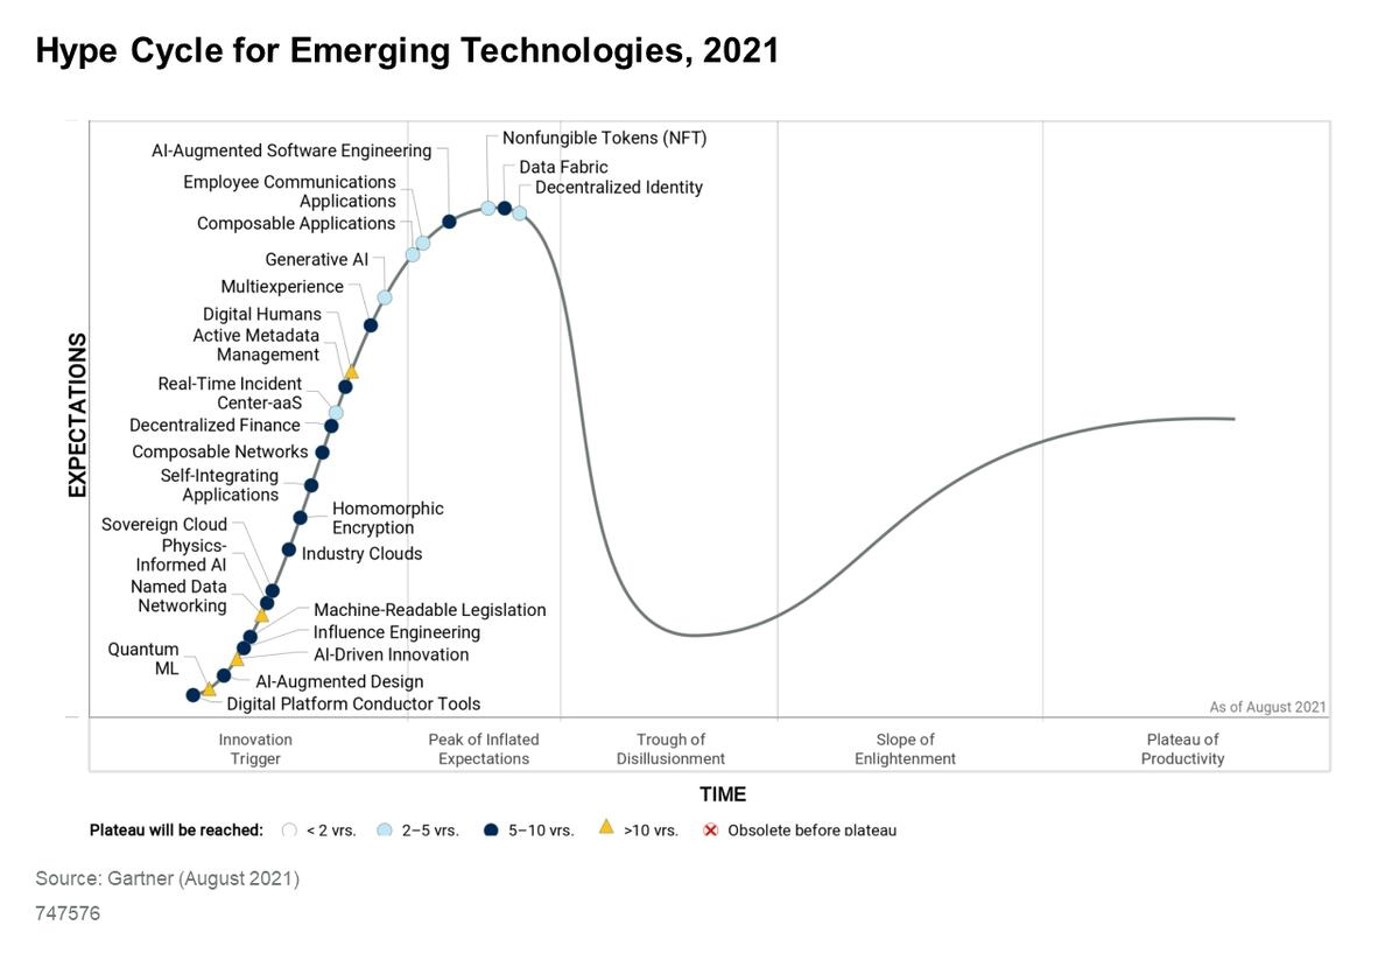
\includegraphics[width=\linewidth,keepaspectratio]{career8}
	\end{center}

\end{frame}

%%%%%%%%%%%%%%%%%%%%%%%%%%%%%%%%%%%%%%%%%%%%%%%%%%%%%%%%%%%
\begin{frame}[fragile]\frametitle{}
	
	\begin{center}
	{\Large Mid-Career Transition to Data Science \ldots}  
	\end{center}

\end{frame}

%%%%%%%%%%%%%%%%%%%%%%%%%%%%%%%%%%%%%%%%%%%%%%%%%%%%%%%%%%%
\begin{frame}[fragile]\frametitle{Pros and Cons}
\begin{columns}
    \begin{column}[T]{0.5\linewidth}
		Advantages:
      \begin{itemize}
			\item Domain Expertise
			\item Maturity, Communication, Soft Skills
			\item Problem Solving
			\end{itemize}
		\end{column}
    \begin{column}[T]{0.5\linewidth}
		
		Dis-advantages:
      \begin{itemize}
			\item Lost touch with Mathematics
			\item Un-Learning and Re-Learning inertia
			\item Starting from scratch? Seniority?
			\end{itemize}
    \end{column}
  \end{columns}
\end{frame}

%%%%%%%%%%%%%%%%%%%%%%%%%%%%%%%%%%%%%%%%%%%%%%%%%%%%%%%%%%%
\begin{frame}[fragile]\frametitle{Why do you want to Switch?}

      \begin{itemize}
			\item $\$_1\$_2\$_3 \ldots \$_n$?
			\item Will remain in fashion forever?
			\item Hate my current job? no growth?
			\end{itemize}
			
			What's in it for me?
\end{frame}

%%%%%%%%%%%%%%%%%%%%%%%%%%%%%%%%%%%%%%%%%%%%%%%%%%%%%%%%%%%
\begin{frame}[fragile]\frametitle{Current + ML combo?}

      \begin{itemize}
			\item First : DON'T QUIT!!!
			\item Don't lose advantage due to domain expertise
			\item ML just another problem solving technique, IF DATA IS AVAILABLE
			\item Can you leverage domain expertise and apply ML there, a good/smooth transition?
			\end{itemize}
			
\end{frame}

%%%%%%%%%%%%%%%%%%%%%%%%%%%%%%%%%%%%%%%%%%%%%%%%%%%%%%%%%%%
\begin{frame}[fragile]\frametitle{}
	
	\begin{center}
	{\Large Learning Path, Roadmap}  
	\end{center}

\end{frame}


%%%%%%%%%%%%%%%%%%%%%%%%%%%%%%%%%%%%%%%%%%%%%%%%%%%%%%%%%%%
\begin{frame}[fragile]\frametitle{Resources}

      \begin{itemize}
			\item First : try Free Online resources, see how much you grasp
			\item No expensive (read, fees in lakhs) certification courses, to start with
			\item Test waters, gain some understanding of yourself then decide.
			\end{itemize}
			
\end{frame}

%%%%%%%%%%%%%%%%%%%%%%%%%%%%%%%%%%%%%%%%%%%%%%%%%%%%%%%%%%%
\begin{frame}[fragile]\frametitle{Steps}

Prep:
      \begin{itemize}
			\item Mathematics: Statistics, Calculus, Linear Algebra
			\item Programming: Python, Data Structure \& Algorithms, Tools
			\item ML/DL: algorithms \& frameworks
			\end{itemize}
			
Practice: Kaggle, Hackathons, projects on Github, blogs, Meetups-talks, etc.
			
\end{frame}

%%%%%%%%%%%%%%%%%%%%%%%%%%%%%%%%%%%%%%%%%%%%%%%%%%%%%%%%%%%
\begin{frame}[fragile]\frametitle{Analytics Vidhya Learning Path 2017}
\begin{columns}
    \begin{column}[T]{0.5\linewidth}
      \begin{itemize}
			\item An year long schedule
			\item Mostly free resources
			\item Followed it myself
			\item Separate paths for:
			      \begin{itemize}

						\item Beginner: Not much experience in programming but just college maths
						\item Transitioner: Decent experience programming, but no ML and just college maths
						\item Intermediate: Knows ML, comfortable with programming and maths.
						\end{itemize}
			\end{itemize}
				https://www.analyticsvidhya.com/blog/2017/01/the-most-comprehensive-data-science-learning-plan-for-2017/

		\end{column}
    \begin{column}[T]{0.5\linewidth}
		
	\begin{center}
	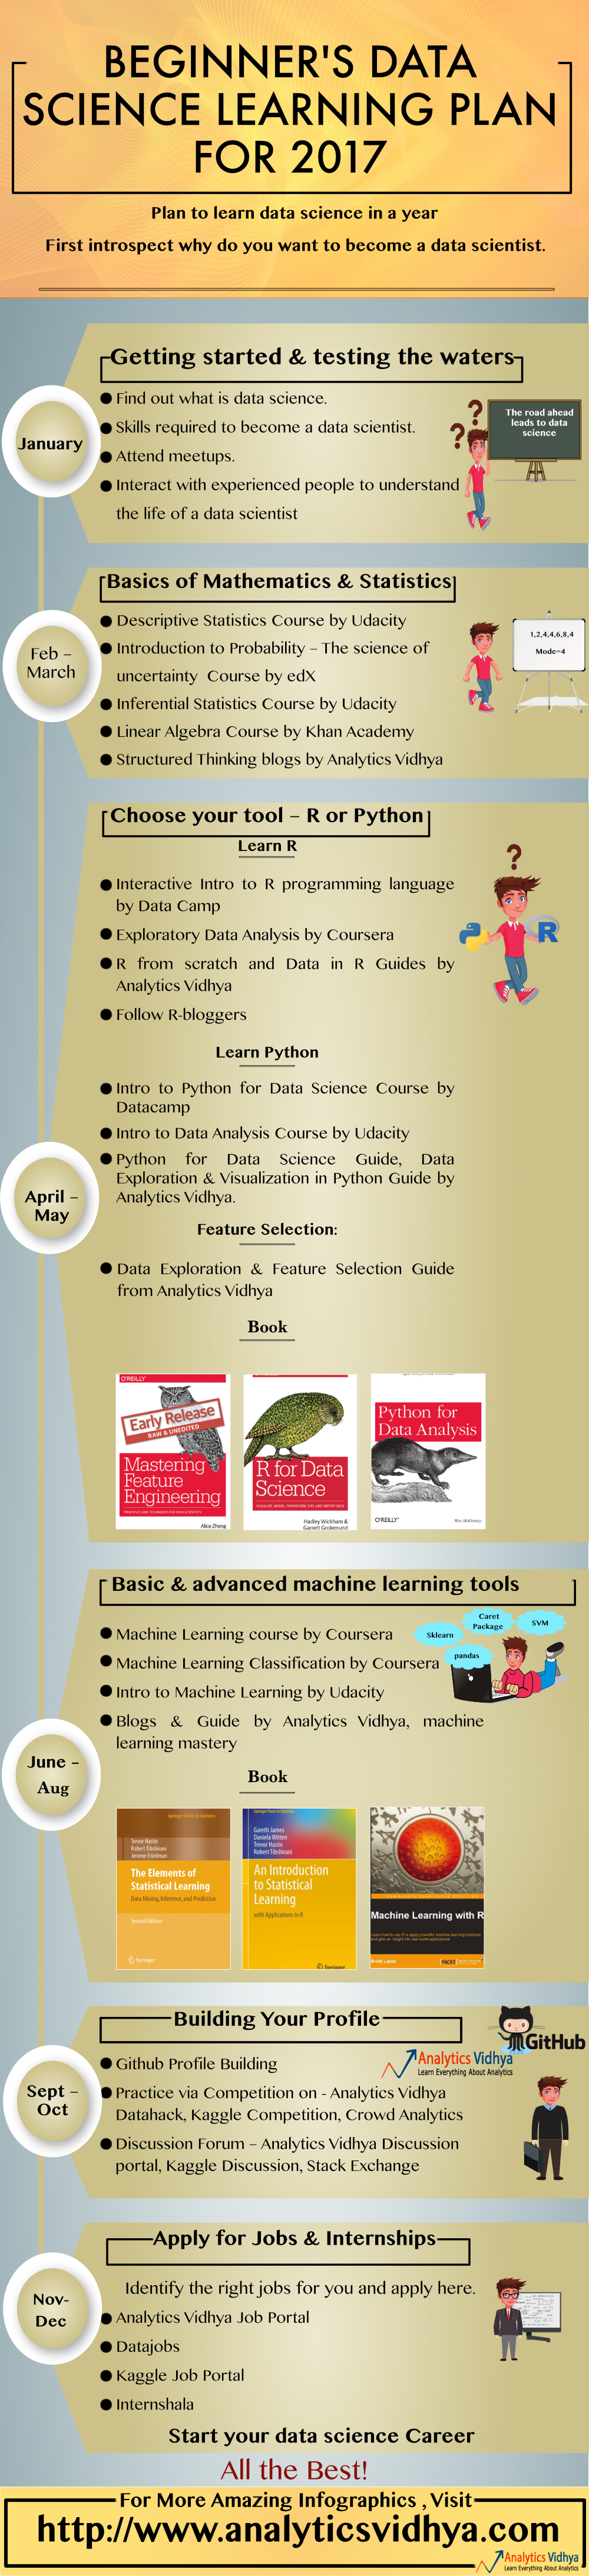
\includegraphics[width=0.3\linewidth,keepaspectratio]{career11}
	\end{center}
    \end{column}
  \end{columns}
	

	
\end{frame}

%%%%%%%%%%%%%%%%%%%%%%%%%%%%%%%%%%%%%%%%%%%%%%%%%%%%%%%%%%%
\begin{frame}[fragile]\frametitle{}
	
	\begin{center}
	{\Large More Generally \ldots For Career \ldots}  
	\end{center}

\end{frame}


%%%%%%%%%%%%%%%%%%%%%%%%%%%%%%%%%%%%%%%%%%%%%%%%%%%%%%%%%%%
\begin{frame}[fragile]\frametitle{Ikigai}
	
	\begin{center}
	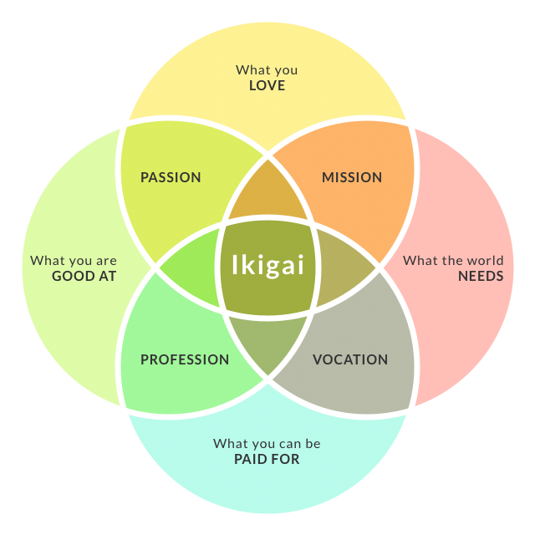
\includegraphics[width=0.6\linewidth,keepaspectratio]{career9}
	\end{center}
	
	{\tiny (Source:  How To Find Your Ikigai And Transform Your Outlook On Life And Business - Chris Myers)}

\end{frame}

%%%%%%%%%%%%%%%%%%%%%%%%%%%%%%%%%%%%%%%%%%%%%%%%%%%%%%%%%%%
\begin{frame}[fragile]\frametitle{Generic Gyan}
\begin{columns}
    \begin{column}[T]{0.4\linewidth}
			Specific Knowledge

      \begin{itemize}
			\item Unique, rare combination
			\item Un-trainable, un-scalable
			\item Acquired through apprenticeship
			\end{itemize}
			
			Leverage
      \begin{itemize}
			\item Permission-ed: Capital, Labor
			\item Un-permission-ed: Content, code
			\item Marginal cost of duplication
			\end{itemize}
			
			Wealth is a positive sum game
			
    \end{column}
    \begin{column}[T]{0.6\linewidth}
		
			\begin{center}
			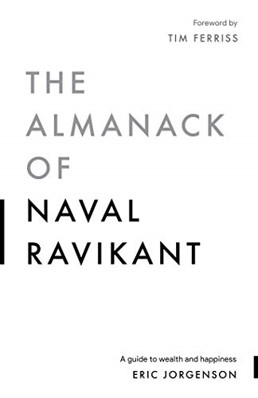
\includegraphics[width=0.4\linewidth,keepaspectratio]{career10}
			\end{center}

			Own story
      \begin{itemize}
			\item Current jobs were not available 10 yrs back
			\item Pick difficult problems/domain, Job, RnD
			\item If not now, can change later, Mid career change, harder, but possible.
			\end{itemize}		
    \end{column}
  \end{columns}
	
\end{frame}

%%%%%%%%%%%%%%%%%%%%%%%%%%%%%%%%%%%%%%%%%%%%%%%%%%%%%%%%%%%
\begin{frame}[fragile]\frametitle{References}
\begin{itemize}
\item Learning Plan 2017 for beginners in data science - Analytics Vidhya
\item What is Data Science? - SimpliLearn
\item Roadmap: How to Learn Machine Learning in 6 Months -  Zach Miller, Senior Data Scientist at Metis
\item Tetiana Ivanova: How to become a Data Scientist in 6 months | PyData London 2016
\item Renee Teate | Becoming a Data Scientist Advice From My Podcast Guests
\item How to switch career to data science from non computer science background - Codebasics
\item Step by step roadmap for machine learning engineer - Codebasics
\item And \ldots Mid-Career Transitions into ML-AI, with Yogesh Kulkarni - Choose To Thinq
\end{itemize}
\end{frame}


%%%%%%%%%%%%%%%%%%%%%%%%%%%%%%%%%%%%%%%%%%%%%%%%%%%%%%%%%%%
\begin{frame}[fragile]\frametitle{}
	
	\begin{center}
	{\Large All the Best!!}
	\end{center}
	
\end{frame}
